\documentclass[]{elsarticle} %review=doublespace preprint=single 5p=2 column
%%% Begin My package additions %%%%%%%%%%%%%%%%%%%
\usepackage[hyphens]{url}

  \journal{An awesome journal} % Sets Journal name


\usepackage{lineno} % add
\providecommand{\tightlist}{%
  \setlength{\itemsep}{0pt}\setlength{\parskip}{0pt}}

\usepackage{graphicx}
\usepackage{booktabs} % book-quality tables
%%%%%%%%%%%%%%%% end my additions to header

\usepackage[T1]{fontenc}
\usepackage{lmodern}
\usepackage{amssymb,amsmath}
\usepackage{ifxetex,ifluatex}
\usepackage{fixltx2e} % provides \textsubscript
% use upquote if available, for straight quotes in verbatim environments
\IfFileExists{upquote.sty}{\usepackage{upquote}}{}
\ifnum 0\ifxetex 1\fi\ifluatex 1\fi=0 % if pdftex
  \usepackage[utf8]{inputenc}
\else % if luatex or xelatex
  \usepackage{fontspec}
  \ifxetex
    \usepackage{xltxtra,xunicode}
  \fi
  \defaultfontfeatures{Mapping=tex-text,Scale=MatchLowercase}
  \newcommand{\euro}{€}
\fi
% use microtype if available
\IfFileExists{microtype.sty}{\usepackage{microtype}}{}
\bibliographystyle{elsarticle-harv}
\usepackage{longtable}
\usepackage{graphicx}
% We will generate all images so they have a width \maxwidth. This means
% that they will get their normal width if they fit onto the page, but
% are scaled down if they would overflow the margins.
\makeatletter
\def\maxwidth{\ifdim\Gin@nat@width>\linewidth\linewidth
\else\Gin@nat@width\fi}
\makeatother
\let\Oldincludegraphics\includegraphics
\renewcommand{\includegraphics}[1]{\Oldincludegraphics[width=\maxwidth]{#1}}
\ifxetex
  \usepackage[setpagesize=false, % page size defined by xetex
              unicode=false, % unicode breaks when used with xetex
              xetex]{hyperref}
\else
  \usepackage[unicode=true]{hyperref}
\fi
\hypersetup{breaklinks=true,
            bookmarks=true,
            pdfauthor={},
            pdftitle={Short Paper},
            colorlinks=false,
            urlcolor=blue,
            linkcolor=magenta,
            pdfborder={0 0 0}}
\urlstyle{same}  % don't use monospace font for urls

\setcounter{secnumdepth}{0}
% Pandoc toggle for numbering sections (defaults to be off)
\setcounter{secnumdepth}{0}


% Pandoc header



\begin{document}
\begin{frontmatter}

  \title{Short Paper}
    \author[Some Institute of Technology]{Alice Anonymous\corref{1}}
   \ead{alice@example.com} 
    \author[Another University]{Bob Security}
   \ead{bob@example.com} 
    \author[Another University]{Cat Memes\corref{2}}
   \ead{cat@example.com} 
    \author[Some Institute of Technology]{Derek Zoolander\corref{2}}
   \ead{derek@example.com} 
      \address[Some Institute of Technology]{Department, Street, City, State, Zip}
    \address[Another University]{Department, Street, City, State, Zip}
      \cortext[1]{Corresponding Author}
    \cortext[2]{Equal contribution}
  
  \begin{abstract}
  This is the abstract.
  
  It consists of two paragraphs.
  \end{abstract}
  
 \end{frontmatter}

\hypertarget{introduction-importing-data}{%
\section{1. Introduction \& Importing
Data}\label{introduction-importing-data}}

We'll work with intraday data for the \emph{S\&P/BMV IPC Equity Index}.
The data consists of \texttt{n\ =\ 2,133,890} observations and
\texttt{k\ =\ 23} variables. The time-series is composed of prices and
trades per minute, spanning from the beginning of 1996 through the first
half of 2018.

First thing we do is take a look at the columns and data types that we
have:

\begin{verbatim}
## Rows: 2,133,890
## Columns: 23
## $ `#RIC`                  <chr> ".MXX", ".MXX", ".MXX", ".MXX", ".MXX", ".M...
## $ `Date[L]`               <dbl> 19960102, 19960102, 19960102, 19960102, 199...
## $ `Time[L]`               <time> 08:36:00, 08:38:00, 08:39:00, 08:40:00, 08...
## $ Type                    <chr> "Intraday 1Min", "Intraday 1Min", "Intraday...
## $ Open                    <dbl> 2777.47, 2777.47, 2777.47, 2777.47, 2777.47...
## $ High                    <dbl> 2777.47, 2777.47, 2777.47, 2777.47, 2777.47...
## $ Low                     <dbl> 2777.47, 2777.47, 2777.47, 2777.47, 2777.14...
## $ Last                    <dbl> 2777.47, 2777.47, 2777.47, 2777.47, 2777.14...
## $ Volume                  <dbl> 0, 0, 0, 0, 0, 0, 0, 0, 0, 0, 0, 0, 0, 0, 0...
## $ `Ave. Price`            <dbl> 2777.470, 2777.470, 2777.470, 2777.470, 277...
## $ VWAP                    <lgl> NA, NA, NA, NA, NA, NA, NA, NA, NA, NA, NA,...
## $ `No. Trades`            <dbl> 1, 2, 3, 3, 3, 3, 3, 3, 3, 3, 3, 3, 3, 2, 3...
## $ `Correction Qualifiers` <lgl> NA, NA, NA, NA, NA, NA, NA, NA, NA, NA, NA,...
## $ `Open Bid`              <lgl> NA, NA, NA, NA, NA, NA, NA, NA, NA, NA, NA,...
## $ `High Bid`              <lgl> NA, NA, NA, NA, NA, NA, NA, NA, NA, NA, NA,...
## $ `Low Bid`               <lgl> NA, NA, NA, NA, NA, NA, NA, NA, NA, NA, NA,...
## $ `Close Bid`             <lgl> NA, NA, NA, NA, NA, NA, NA, NA, NA, NA, NA,...
## $ `No. Bids`              <dbl> 0, 0, 0, 0, 0, 0, 0, 0, 0, 0, 0, 0, 0, 0, 0...
## $ `Open Ask`              <lgl> NA, NA, NA, NA, NA, NA, NA, NA, NA, NA, NA,...
## $ `High Ask`              <lgl> NA, NA, NA, NA, NA, NA, NA, NA, NA, NA, NA,...
## $ `Low Ask`               <lgl> NA, NA, NA, NA, NA, NA, NA, NA, NA, NA, NA,...
## $ `Close Ask`             <lgl> NA, NA, NA, NA, NA, NA, NA, NA, NA, NA, NA,...
## $ `No. Asks`              <dbl> 0, 0, 0, 0, 0, 0, 0, 0, 0, 0, 0, 0, 0, 0, 0...
\end{verbatim}

We can count how many \texttt{NA}s are present in our data. We do this
per column:

\begin{verbatim}
## Rows: 1
## Columns: 23
## $ ticker                <int> 0
## $ raw_date              <int> 0
## $ raw_time              <int> 0
## $ type                  <int> 0
## $ open                  <int> 0
## $ high                  <int> 0
## $ low                   <int> 0
## $ last                  <int> 0
## $ volume                <int> 0
## $ average_price         <int> 0
## $ vwap                  <int> 2133890
## $ no_trades             <int> 0
## $ correction_qualifiers <int> 2133890
## $ open_bid              <int> 2133890
## $ high_bid              <int> 2133890
## $ low_bid               <int> 2133890
## $ close_bid             <int> 2133890
## $ no_bids               <int> 0
## $ open_ask              <int> 2133890
## $ high_ask              <int> 2133890
## $ low_ask               <int> 2133890
## $ close_ask             <int> 2133890
## $ no_ask                <int> 0
\end{verbatim}

We see that there are 10 columns (variables) that have all values as
\texttt{NA}. We assign these variables to the
\texttt{columns\_to\_remove} object and remove them from the data.

\begin{verbatim}
##  [1] "vwap"                  "correction_qualifiers" "open_bid"             
##  [4] "high_bid"              "low_bid"               "close_bid"            
##  [7] "open_ask"              "high_ask"              "low_ask"              
## [10] "close_ask"
\end{verbatim}

We name the \emph{clean} dataset as \texttt{IPC\_ip} (IPC intraday
prices) and again see the column names and each data type.

\begin{verbatim}
## Rows: 2,133,890
## Columns: 13
## $ ticker        <chr> ".MXX", ".MXX", ".MXX", ".MXX", ".MXX", ".MXX", ".MXX...
## $ raw_date      <dbl> 19960102, 19960102, 19960102, 19960102, 19960102, 199...
## $ raw_time      <time> 08:36:00, 08:38:00, 08:39:00, 08:40:00, 08:41:00, 08...
## $ type          <chr> "Intraday 1Min", "Intraday 1Min", "Intraday 1Min", "I...
## $ open          <dbl> 2777.47, 2777.47, 2777.47, 2777.47, 2777.47, 2777.14,...
## $ high          <dbl> 2777.47, 2777.47, 2777.47, 2777.47, 2777.47, 2777.14,...
## $ low           <dbl> 2777.47, 2777.47, 2777.47, 2777.47, 2777.14, 2777.14,...
## $ last          <dbl> 2777.47, 2777.47, 2777.47, 2777.47, 2777.14, 2777.14,...
## $ volume        <dbl> 0, 0, 0, 0, 0, 0, 0, 0, 0, 0, 0, 0, 0, 0, 0, 0, 0, 0,...
## $ average_price <dbl> 2777.470, 2777.470, 2777.470, 2777.470, 2777.360, 277...
## $ no_trades     <dbl> 1, 2, 3, 3, 3, 3, 3, 3, 3, 3, 3, 3, 3, 2, 3, 3, 3, 3,...
## $ no_bids       <dbl> 0, 0, 0, 0, 0, 0, 0, 0, 0, 0, 0, 0, 0, 0, 0, 0, 0, 0,...
## $ no_ask        <dbl> 0, 0, 0, 0, 0, 0, 0, 0, 0, 0, 0, 0, 0, 0, 0, 0, 0, 0,...
\end{verbatim}

\hypertarget{feature-engineering-data-wrangling}{%
\section{2. Feature Engineering \& Data
Wrangling}\label{feature-engineering-data-wrangling}}

We then carry on with the analysis by creating some new variables
(a.k.a. \emph{Feature Engineering}) and manipulating the data.

First, we create a \texttt{tidy\_date} variable where we store the date
according to the \emph{ISO 8601} standard that states that dates should
be expressed in the \texttt{YYYY-MM-DD} format. In consequence, the
\texttt{raw\_date} column is dropped and we keep the newly created
\texttt{tidy\_date} variable instead.

Also, we drop the \texttt{ticker}, \texttt{type}, \texttt{open},
\texttt{high}, and \texttt{low} columns because we think they are of no
use for the analysis.

We store the modified data into the \texttt{IPC\_tbl} (IPC tibble)
object.

\hypertarget{time-series-data-print}{%
\subsubsection{Time-Series Data Print}\label{time-series-data-print}}

Next, we create some time-related variables, such as:

\texttt{tidy\_year}: a \texttt{dbl} that stores the year (from 1996 -
2018).

\texttt{tidy\_month}: a \texttt{dbl} that stores the month as a number
(from 1 through 12).

\texttt{tidy\_mday}: a \texttt{dbl} that stores the day number within
each month (from 1 through 31).

\texttt{tidy\_wday}: a categorical variable (\texttt{fctr}) that
includes: \texttt{Mon} \texttt{Tue} \texttt{Wed} \texttt{Thu}
\texttt{Fri}.

\texttt{tidy\_hour}: a \texttt{dbl} that stores the hour (we have data
from 5 through 20 hours).

\texttt{tidy\_minute}: a \texttt{dbl} that stores the minute of the
trade (from 0 through 59).

\texttt{tidy\_time}: an \texttt{hms} (hour-minute-second) object that
stores the time of the trade.

\begin{longtable}[]{@{}ll@{}}
\caption{Data summary}\tabularnewline
\toprule
\endhead
Name & Piped data\tabularnewline
Number of rows & 2133890\tabularnewline
Number of columns & 15\tabularnewline
\_\_\_\_\_\_\_\_\_\_\_\_\_\_\_\_\_\_\_\_\_\_\_ &\tabularnewline
Column type frequency: &\tabularnewline
Date & 1\tabularnewline
difftime & 1\tabularnewline
factor & 1\tabularnewline
numeric & 12\tabularnewline
\_\_\_\_\_\_\_\_\_\_\_\_\_\_\_\_\_\_\_\_\_\_\_\_ &\tabularnewline
Group variables & None\tabularnewline
\bottomrule
\end{longtable}

\textbf{Variable type: Date}

\begin{longtable}[]{@{}lrrlllr@{}}
\toprule
skim\_variable & n\_missing & complete\_rate & min & max & median &
n\_unique\tabularnewline
\midrule
\endhead
tidy\_date & 0 & 1 & 1996-01-02 & 2018-06-05 & 2007-07-25 &
5613\tabularnewline
\bottomrule
\end{longtable}

\textbf{Variable type: difftime}

\begin{longtable}[]{@{}lrrlllr@{}}
\toprule
skim\_variable & n\_missing & complete\_rate & min & max & median &
n\_unique\tabularnewline
\midrule
\endhead
tidy\_time & 0 & 1 & 19920 secs & 73320 secs & 42300 secs &
647\tabularnewline
\bottomrule
\end{longtable}

\textbf{Variable type: factor}

\begin{longtable}[]{@{}lrrlrl@{}}
\toprule
skim\_variable & n\_missing & complete\_rate & ordered & n\_unique &
top\_counts\tabularnewline
\midrule
\endhead
tidy\_wday & 0 & 1 & TRUE & 5 & Wed: 435537, Tue: 434397, Thu: 426174,
Fri: 425693\tabularnewline
\bottomrule
\end{longtable}

\textbf{Variable type: numeric}

\begin{longtable}[]{@{}lrrrrrrrrrl@{}}
\toprule
\begin{minipage}[b]{0.06\columnwidth}\raggedright
skim\_variable\strut
\end{minipage} & \begin{minipage}[b]{0.04\columnwidth}\raggedleft
n\_missing\strut
\end{minipage} & \begin{minipage}[b]{0.06\columnwidth}\raggedleft
complete\_rate\strut
\end{minipage} & \begin{minipage}[b]{0.05\columnwidth}\raggedleft
mean\strut
\end{minipage} & \begin{minipage}[b]{0.05\columnwidth}\raggedleft
sd\strut
\end{minipage} & \begin{minipage}[b]{0.04\columnwidth}\raggedleft
p0\strut
\end{minipage} & \begin{minipage}[b]{0.05\columnwidth}\raggedleft
p25\strut
\end{minipage} & \begin{minipage}[b]{0.05\columnwidth}\raggedleft
p50\strut
\end{minipage} & \begin{minipage}[b]{0.05\columnwidth}\raggedleft
p75\strut
\end{minipage} & \begin{minipage}[b]{0.06\columnwidth}\raggedleft
p100\strut
\end{minipage} & \begin{minipage}[b]{0.18\columnwidth}\raggedright
hist\strut
\end{minipage}\tabularnewline
\midrule
\endhead
\begin{minipage}[t]{0.06\columnwidth}\raggedright
trade\_id\strut
\end{minipage} & \begin{minipage}[t]{0.04\columnwidth}\raggedleft
0\strut
\end{minipage} & \begin{minipage}[t]{0.06\columnwidth}\raggedleft
1\strut
\end{minipage} & \begin{minipage}[t]{0.05\columnwidth}\raggedleft
1066945.50\strut
\end{minipage} & \begin{minipage}[t]{0.05\columnwidth}\raggedleft
616001.13\strut
\end{minipage} & \begin{minipage}[t]{0.04\columnwidth}\raggedleft
1.00\strut
\end{minipage} & \begin{minipage}[t]{0.05\columnwidth}\raggedleft
533473.25\strut
\end{minipage} & \begin{minipage}[t]{0.05\columnwidth}\raggedleft
1066945.50\strut
\end{minipage} & \begin{minipage}[t]{0.05\columnwidth}\raggedleft
1600417.75\strut
\end{minipage} & \begin{minipage}[t]{0.06\columnwidth}\raggedleft
2.133890e+06\strut
\end{minipage} & \begin{minipage}[t]{0.18\columnwidth}\raggedright
▇▇▇▇▇\strut
\end{minipage}\tabularnewline
\begin{minipage}[t]{0.06\columnwidth}\raggedright
last\strut
\end{minipage} & \begin{minipage}[t]{0.04\columnwidth}\raggedleft
0\strut
\end{minipage} & \begin{minipage}[t]{0.06\columnwidth}\raggedleft
1\strut
\end{minipage} & \begin{minipage}[t]{0.05\columnwidth}\raggedleft
23945.92\strut
\end{minipage} & \begin{minipage}[t]{0.05\columnwidth}\raggedleft
16340.42\strut
\end{minipage} & \begin{minipage}[t]{0.04\columnwidth}\raggedleft
2731.21\strut
\end{minipage} & \begin{minipage}[t]{0.05\columnwidth}\raggedleft
6502.76\strut
\end{minipage} & \begin{minipage}[t]{0.05\columnwidth}\raggedleft
24198.56\strut
\end{minipage} & \begin{minipage}[t]{0.05\columnwidth}\raggedleft
40435.79\strut
\end{minipage} & \begin{minipage}[t]{0.06\columnwidth}\raggedleft
7.813872e+04\strut
\end{minipage} & \begin{minipage}[t]{0.18\columnwidth}\raggedright
▇▃▆▁▁\strut
\end{minipage}\tabularnewline
\begin{minipage}[t]{0.06\columnwidth}\raggedright
volume\strut
\end{minipage} & \begin{minipage}[t]{0.04\columnwidth}\raggedleft
0\strut
\end{minipage} & \begin{minipage}[t]{0.06\columnwidth}\raggedleft
1\strut
\end{minipage} & \begin{minipage}[t]{0.05\columnwidth}\raggedleft
55341101.47\strut
\end{minipage} & \begin{minipage}[t]{0.05\columnwidth}\raggedleft
54169304.82\strut
\end{minipage} & \begin{minipage}[t]{0.04\columnwidth}\raggedleft
0.00\strut
\end{minipage} & \begin{minipage}[t]{0.05\columnwidth}\raggedleft
11697950.75\strut
\end{minipage} & \begin{minipage}[t]{0.05\columnwidth}\raggedleft
42617270.00\strut
\end{minipage} & \begin{minipage}[t]{0.05\columnwidth}\raggedleft
83705131.25\strut
\end{minipage} & \begin{minipage}[t]{0.06\columnwidth}\raggedleft
1.759968e+09\strut
\end{minipage} & \begin{minipage}[t]{0.18\columnwidth}\raggedright
▇▁▁▁▁\strut
\end{minipage}\tabularnewline
\begin{minipage}[t]{0.06\columnwidth}\raggedright
average\_price\strut
\end{minipage} & \begin{minipage}[t]{0.04\columnwidth}\raggedleft
0\strut
\end{minipage} & \begin{minipage}[t]{0.06\columnwidth}\raggedleft
1\strut
\end{minipage} & \begin{minipage}[t]{0.05\columnwidth}\raggedleft
23945.91\strut
\end{minipage} & \begin{minipage}[t]{0.05\columnwidth}\raggedleft
16340.43\strut
\end{minipage} & \begin{minipage}[t]{0.04\columnwidth}\raggedleft
2731.36\strut
\end{minipage} & \begin{minipage}[t]{0.05\columnwidth}\raggedleft
6502.69\strut
\end{minipage} & \begin{minipage}[t]{0.05\columnwidth}\raggedleft
24199.01\strut
\end{minipage} & \begin{minipage}[t]{0.05\columnwidth}\raggedleft
40435.50\strut
\end{minipage} & \begin{minipage}[t]{0.06\columnwidth}\raggedleft
7.813872e+04\strut
\end{minipage} & \begin{minipage}[t]{0.18\columnwidth}\raggedright
▇▃▆▁▁\strut
\end{minipage}\tabularnewline
\begin{minipage}[t]{0.06\columnwidth}\raggedright
no\_trades\strut
\end{minipage} & \begin{minipage}[t]{0.04\columnwidth}\raggedleft
0\strut
\end{minipage} & \begin{minipage}[t]{0.06\columnwidth}\raggedleft
1\strut
\end{minipage} & \begin{minipage}[t]{0.05\columnwidth}\raggedleft
34.98\strut
\end{minipage} & \begin{minipage}[t]{0.05\columnwidth}\raggedleft
39.95\strut
\end{minipage} & \begin{minipage}[t]{0.04\columnwidth}\raggedleft
1.00\strut
\end{minipage} & \begin{minipage}[t]{0.05\columnwidth}\raggedleft
8.00\strut
\end{minipage} & \begin{minipage}[t]{0.05\columnwidth}\raggedleft
21.00\strut
\end{minipage} & \begin{minipage}[t]{0.05\columnwidth}\raggedleft
53.00\strut
\end{minipage} & \begin{minipage}[t]{0.06\columnwidth}\raggedleft
3.693000e+03\strut
\end{minipage} & \begin{minipage}[t]{0.18\columnwidth}\raggedright
▇▁▁▁▁\strut
\end{minipage}\tabularnewline
\begin{minipage}[t]{0.06\columnwidth}\raggedright
no\_bids\strut
\end{minipage} & \begin{minipage}[t]{0.04\columnwidth}\raggedleft
0\strut
\end{minipage} & \begin{minipage}[t]{0.06\columnwidth}\raggedleft
1\strut
\end{minipage} & \begin{minipage}[t]{0.05\columnwidth}\raggedleft
0.00\strut
\end{minipage} & \begin{minipage}[t]{0.05\columnwidth}\raggedleft
0.00\strut
\end{minipage} & \begin{minipage}[t]{0.04\columnwidth}\raggedleft
0.00\strut
\end{minipage} & \begin{minipage}[t]{0.05\columnwidth}\raggedleft
0.00\strut
\end{minipage} & \begin{minipage}[t]{0.05\columnwidth}\raggedleft
0.00\strut
\end{minipage} & \begin{minipage}[t]{0.05\columnwidth}\raggedleft
0.00\strut
\end{minipage} & \begin{minipage}[t]{0.06\columnwidth}\raggedleft
0.000000e+00\strut
\end{minipage} & \begin{minipage}[t]{0.18\columnwidth}\raggedright
▁▁▇▁▁\strut
\end{minipage}\tabularnewline
\begin{minipage}[t]{0.06\columnwidth}\raggedright
no\_ask\strut
\end{minipage} & \begin{minipage}[t]{0.04\columnwidth}\raggedleft
0\strut
\end{minipage} & \begin{minipage}[t]{0.06\columnwidth}\raggedleft
1\strut
\end{minipage} & \begin{minipage}[t]{0.05\columnwidth}\raggedleft
0.00\strut
\end{minipage} & \begin{minipage}[t]{0.05\columnwidth}\raggedleft
0.00\strut
\end{minipage} & \begin{minipage}[t]{0.04\columnwidth}\raggedleft
0.00\strut
\end{minipage} & \begin{minipage}[t]{0.05\columnwidth}\raggedleft
0.00\strut
\end{minipage} & \begin{minipage}[t]{0.05\columnwidth}\raggedleft
0.00\strut
\end{minipage} & \begin{minipage}[t]{0.05\columnwidth}\raggedleft
0.00\strut
\end{minipage} & \begin{minipage}[t]{0.06\columnwidth}\raggedleft
0.000000e+00\strut
\end{minipage} & \begin{minipage}[t]{0.18\columnwidth}\raggedright
▁▁▇▁▁\strut
\end{minipage}\tabularnewline
\begin{minipage}[t]{0.06\columnwidth}\raggedright
tidy\_year\strut
\end{minipage} & \begin{minipage}[t]{0.04\columnwidth}\raggedleft
0\strut
\end{minipage} & \begin{minipage}[t]{0.06\columnwidth}\raggedleft
1\strut
\end{minipage} & \begin{minipage}[t]{0.05\columnwidth}\raggedleft
2007.00\strut
\end{minipage} & \begin{minipage}[t]{0.05\columnwidth}\raggedleft
6.39\strut
\end{minipage} & \begin{minipage}[t]{0.04\columnwidth}\raggedleft
1996.00\strut
\end{minipage} & \begin{minipage}[t]{0.05\columnwidth}\raggedleft
2002.00\strut
\end{minipage} & \begin{minipage}[t]{0.05\columnwidth}\raggedleft
2007.00\strut
\end{minipage} & \begin{minipage}[t]{0.05\columnwidth}\raggedleft
2013.00\strut
\end{minipage} & \begin{minipage}[t]{0.06\columnwidth}\raggedleft
2.018000e+03\strut
\end{minipage} & \begin{minipage}[t]{0.18\columnwidth}\raggedright
▇▆▇▆▇\strut
\end{minipage}\tabularnewline
\begin{minipage}[t]{0.06\columnwidth}\raggedright
tidy\_month\strut
\end{minipage} & \begin{minipage}[t]{0.04\columnwidth}\raggedleft
0\strut
\end{minipage} & \begin{minipage}[t]{0.06\columnwidth}\raggedleft
1\strut
\end{minipage} & \begin{minipage}[t]{0.05\columnwidth}\raggedleft
6.43\strut
\end{minipage} & \begin{minipage}[t]{0.05\columnwidth}\raggedleft
3.43\strut
\end{minipage} & \begin{minipage}[t]{0.04\columnwidth}\raggedleft
1.00\strut
\end{minipage} & \begin{minipage}[t]{0.05\columnwidth}\raggedleft
3.00\strut
\end{minipage} & \begin{minipage}[t]{0.05\columnwidth}\raggedleft
6.00\strut
\end{minipage} & \begin{minipage}[t]{0.05\columnwidth}\raggedleft
9.00\strut
\end{minipage} & \begin{minipage}[t]{0.06\columnwidth}\raggedleft
1.200000e+01\strut
\end{minipage} & \begin{minipage}[t]{0.18\columnwidth}\raggedright
▇▅▆▅▇\strut
\end{minipage}\tabularnewline
\begin{minipage}[t]{0.06\columnwidth}\raggedright
tidy\_mday\strut
\end{minipage} & \begin{minipage}[t]{0.04\columnwidth}\raggedleft
0\strut
\end{minipage} & \begin{minipage}[t]{0.06\columnwidth}\raggedleft
1\strut
\end{minipage} & \begin{minipage}[t]{0.05\columnwidth}\raggedleft
15.84\strut
\end{minipage} & \begin{minipage}[t]{0.05\columnwidth}\raggedleft
8.75\strut
\end{minipage} & \begin{minipage}[t]{0.04\columnwidth}\raggedleft
1.00\strut
\end{minipage} & \begin{minipage}[t]{0.05\columnwidth}\raggedleft
8.00\strut
\end{minipage} & \begin{minipage}[t]{0.05\columnwidth}\raggedleft
16.00\strut
\end{minipage} & \begin{minipage}[t]{0.05\columnwidth}\raggedleft
23.00\strut
\end{minipage} & \begin{minipage}[t]{0.06\columnwidth}\raggedleft
3.100000e+01\strut
\end{minipage} & \begin{minipage}[t]{0.18\columnwidth}\raggedright
▇▇▇▇▆\strut
\end{minipage}\tabularnewline
\begin{minipage}[t]{0.06\columnwidth}\raggedright
tidy\_hour\strut
\end{minipage} & \begin{minipage}[t]{0.04\columnwidth}\raggedleft
0\strut
\end{minipage} & \begin{minipage}[t]{0.06\columnwidth}\raggedleft
1\strut
\end{minipage} & \begin{minipage}[t]{0.05\columnwidth}\raggedleft
11.24\strut
\end{minipage} & \begin{minipage}[t]{0.05\columnwidth}\raggedleft
1.92\strut
\end{minipage} & \begin{minipage}[t]{0.04\columnwidth}\raggedleft
5.00\strut
\end{minipage} & \begin{minipage}[t]{0.05\columnwidth}\raggedleft
10.00\strut
\end{minipage} & \begin{minipage}[t]{0.05\columnwidth}\raggedleft
11.00\strut
\end{minipage} & \begin{minipage}[t]{0.05\columnwidth}\raggedleft
13.00\strut
\end{minipage} & \begin{minipage}[t]{0.06\columnwidth}\raggedleft
2.000000e+01\strut
\end{minipage} & \begin{minipage}[t]{0.18\columnwidth}\raggedright
▂▇▇▁▁\strut
\end{minipage}\tabularnewline
\begin{minipage}[t]{0.06\columnwidth}\raggedright
tidy\_minute\strut
\end{minipage} & \begin{minipage}[t]{0.04\columnwidth}\raggedleft
0\strut
\end{minipage} & \begin{minipage}[t]{0.06\columnwidth}\raggedleft
1\strut
\end{minipage} & \begin{minipage}[t]{0.05\columnwidth}\raggedleft
30.52\strut
\end{minipage} & \begin{minipage}[t]{0.05\columnwidth}\raggedleft
17.33\strut
\end{minipage} & \begin{minipage}[t]{0.04\columnwidth}\raggedleft
0.00\strut
\end{minipage} & \begin{minipage}[t]{0.05\columnwidth}\raggedleft
16.00\strut
\end{minipage} & \begin{minipage}[t]{0.05\columnwidth}\raggedleft
31.00\strut
\end{minipage} & \begin{minipage}[t]{0.05\columnwidth}\raggedleft
46.00\strut
\end{minipage} & \begin{minipage}[t]{0.06\columnwidth}\raggedleft
5.900000e+01\strut
\end{minipage} & \begin{minipage}[t]{0.18\columnwidth}\raggedright
▇▇▇▇▇\strut
\end{minipage}\tabularnewline
\bottomrule
\end{longtable}

\hypertarget{computing-intraday-log-returns}{%
\subsection{2.1 Computing Intraday
Log-Returns}\label{computing-intraday-log-returns}}

Next, we compute the intraday returns and assign them to the
\texttt{log\_ret} variable. We also convert our data into a
time-friendly type of object called \texttt{tibble\ time} (we do this
via the \texttt{as\_tbl\_time()} function).

\begin{verbatim}
## # A time tibble: 2,133,890 x 16
## # Index: tidy_date
##    trade_id tidy_date   log_ret tidy_time  last volume average_price no_trades
##       <int> <date>        <dbl> <time>    <dbl>  <dbl>         <dbl>     <dbl>
##  1        1 1996-01-02 NA       08:36     2777.      0         2777.         1
##  2        2 1996-01-02  0.      08:38     2777.      0         2777.         2
##  3        3 1996-01-02  0.      08:39     2777.      0         2777.         3
##  4        4 1996-01-02  0.      08:40     2777.      0         2777.         3
##  5        5 1996-01-02 -1.19e-4 08:41     2777.      0         2777.         3
##  6        6 1996-01-02  0.      08:42     2777.      0         2777.         3
##  7        7 1996-01-02  0.      08:43     2777.      0         2777.         3
##  8        8 1996-01-02  0.      08:44     2777.      0         2777.         3
##  9        9 1996-01-02  0.      08:45     2777.      0         2777.         3
## 10       10 1996-01-02  0.      08:46     2777.      0         2777.         3
## # ... with 2,133,880 more rows, and 8 more variables: no_bids <dbl>,
## #   no_ask <dbl>, tidy_year <dbl>, tidy_month <dbl>, tidy_mday <int>,
## #   tidy_wday <ord>, tidy_hour <int>, tidy_minute <int>
\end{verbatim}

\hypertarget{narrowing-down-the-time-window-for-trades}{%
\subsection{2.2 Narrowing down the time window for
trades}\label{narrowing-down-the-time-window-for-trades}}

First, it's useful to see how many different trading-days we have in our
data.

\begin{verbatim}
## [1] 5613
\end{verbatim}

So we have \texttt{5,613} different trading- days.

It's worth noting that, for the \texttt{tidy\_time} variable, we have
data from \texttt{05:32:00} all the way through \texttt{20:22:00}.

Let's see the earliest times in our data:

\begin{verbatim}
## # A tibble: 6 x 1
##   tidy_time
##   <time>   
## 1 05:32    
## 2 05:33    
## 3 06:32    
## 4 06:33    
## 5 06:34    
## 6 06:35
\end{verbatim}

And the latest times in our data:

\begin{verbatim}
## # A tibble: 6 x 1
##   tidy_time
##   <time>   
## 1 20:17    
## 2 20:18    
## 3 20:19    
## 4 20:20    
## 5 20:21    
## 6 20:22
\end{verbatim}

We can also visualize how many datapoints we have, per hour.

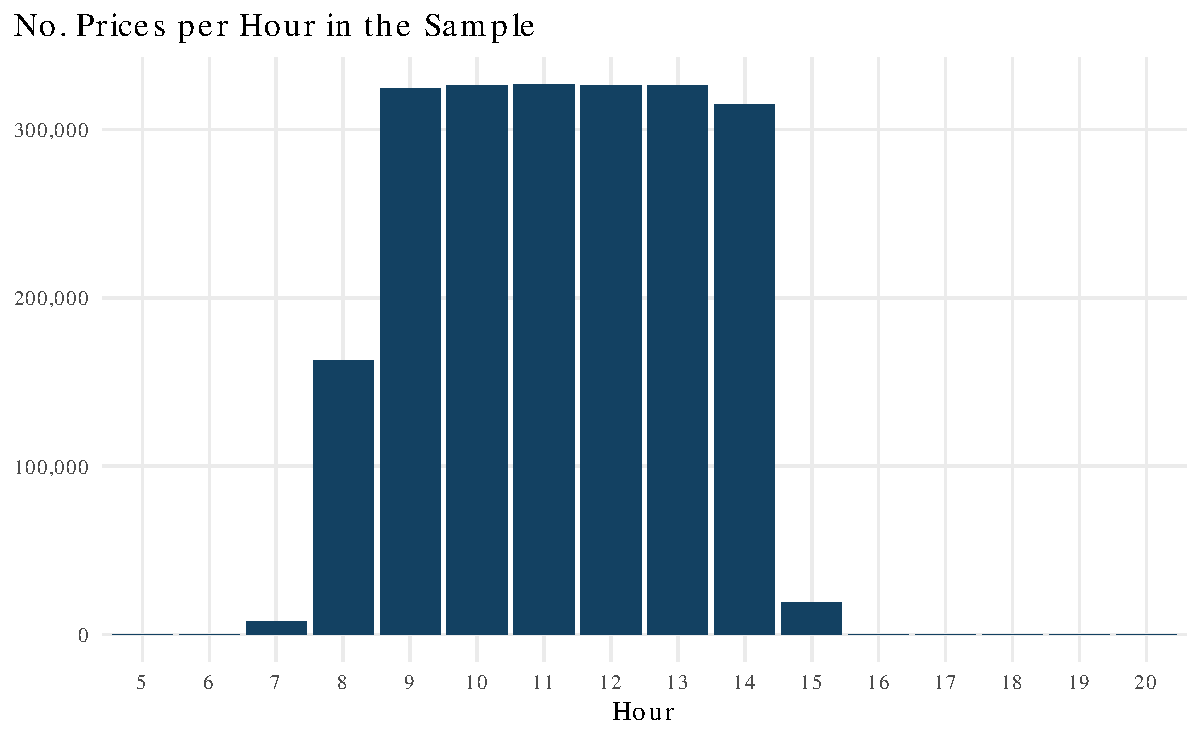
\includegraphics{01-Data-Prep-Elsevier_files/figure-latex/unnamed-chunk-13-1.pdf}

From the plot above, we see that most of the prices lie between 8:00AM -
3:00PM. It's interesting that the hours \texttt{8} and \texttt{15} have
fewer datapoints. We can further inspect each one to see the hour-minute
components of those trades.

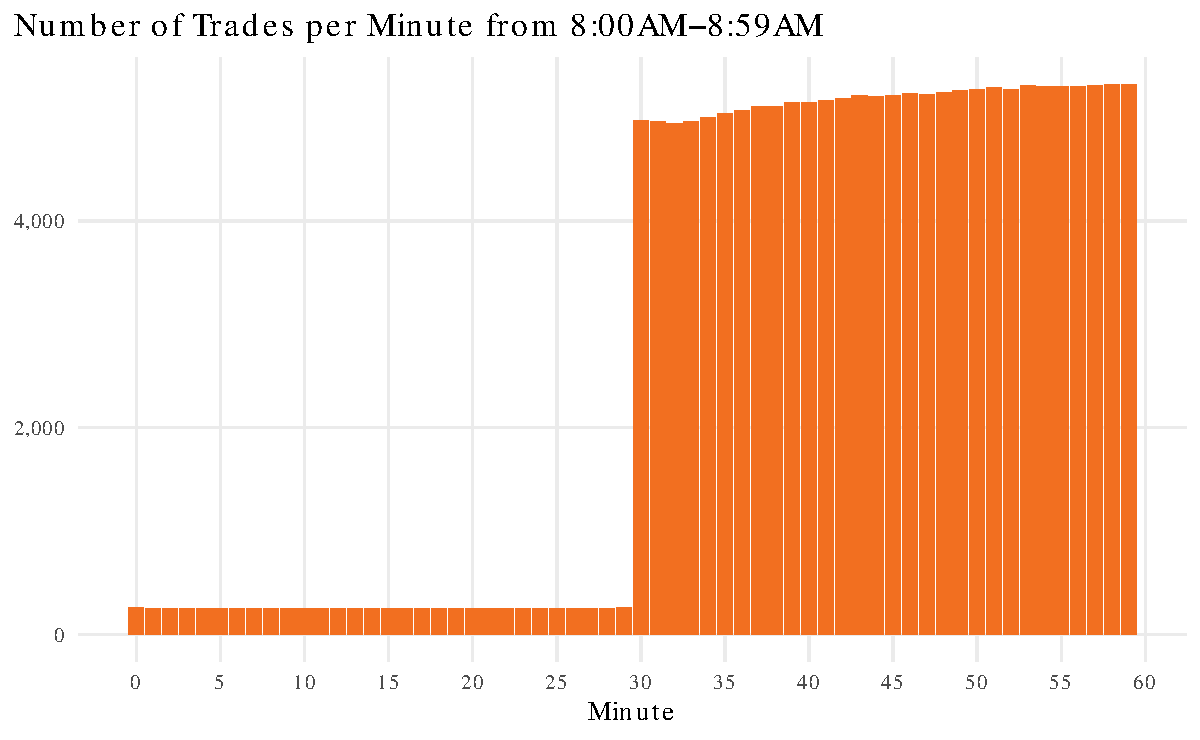
\includegraphics{01-Data-Prep-Elsevier_files/figure-latex/unnamed-chunk-14-1.pdf}

As expected, the second half-hour is the most active (that is, the
period from 8:30AM - 8:59AM).

Now, let's do the same for the \texttt{15} hour-mark:

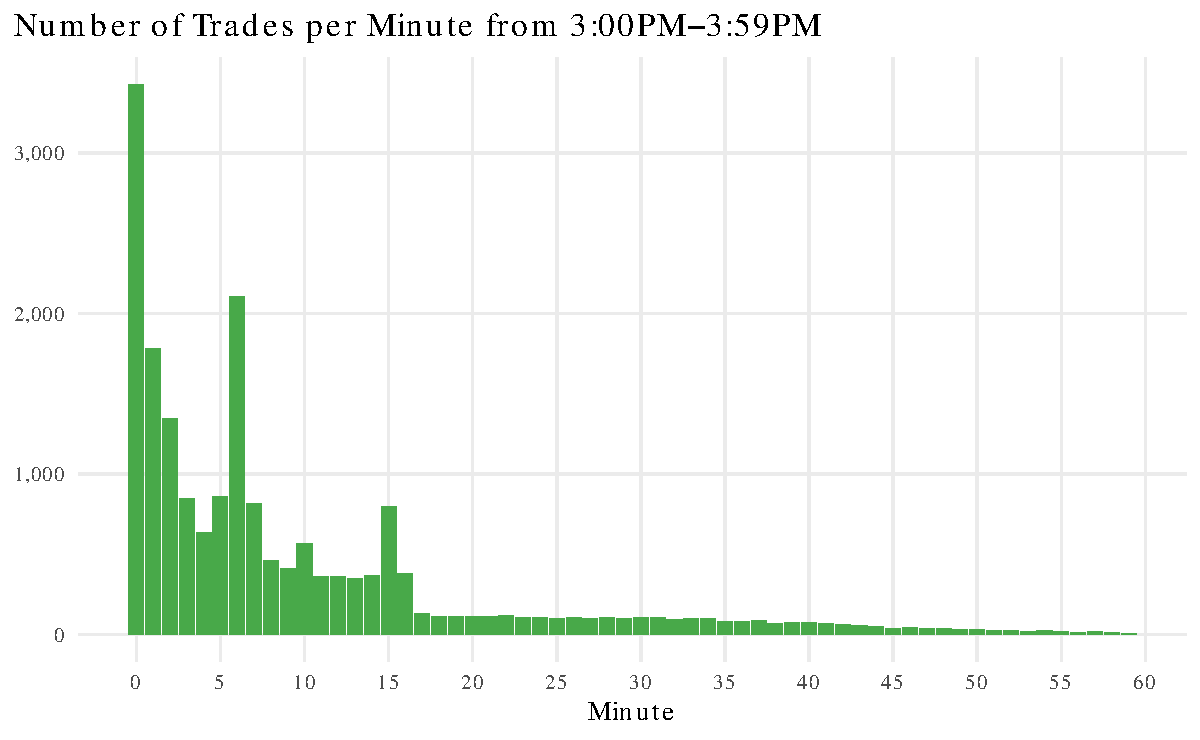
\includegraphics{01-Data-Prep-Elsevier_files/figure-latex/unnamed-chunk-15-1.pdf}

Here, the time with most trades is 3:00PM exactly. That's what we need
because we'll ignore the rest of the trades. Following Liu, Patton,
Sheppard (2013), we'll discard any prices that were quoted outside
normal business hours. Hence, we want trades that lie between
\texttt{08:30} and \texttt{15:00}. We'll store these trades in a new
object called \texttt{IPC\_tfr\_tbl} (IPC time-filtered returns tibble).
Finally, we'll print the earliest and latest times in our data to check.

\begin{verbatim}
## # A time tibble: 2,102,987 x 16
## # Index: tidy_date
##    trade_id tidy_date   log_ret tidy_time  last volume average_price no_trades
##       <int> <date>        <dbl> <time>    <dbl>  <dbl>         <dbl>     <dbl>
##  1        1 1996-01-02 NA       08:36     2777.      0         2777.         1
##  2        2 1996-01-02  0.      08:38     2777.      0         2777.         2
##  3        3 1996-01-02  0.      08:39     2777.      0         2777.         3
##  4        4 1996-01-02  0.      08:40     2777.      0         2777.         3
##  5        5 1996-01-02 -1.19e-4 08:41     2777.      0         2777.         3
##  6        6 1996-01-02  0.      08:42     2777.      0         2777.         3
##  7        7 1996-01-02  0.      08:43     2777.      0         2777.         3
##  8        8 1996-01-02  0.      08:44     2777.      0         2777.         3
##  9        9 1996-01-02  0.      08:45     2777.      0         2777.         3
## 10       10 1996-01-02  0.      08:46     2777.      0         2777.         3
## # ... with 2,102,977 more rows, and 8 more variables: no_bids <dbl>,
## #   no_ask <dbl>, tidy_year <dbl>, tidy_month <dbl>, tidy_mday <int>,
## #   tidy_wday <ord>, tidy_hour <int>, tidy_minute <int>
\end{verbatim}

\begin{verbatim}
## # A tibble: 6 x 1
##   tidy_time
##   <time>   
## 1 08:30    
## 2 08:31    
## 3 08:32    
## 4 08:33    
## 5 08:34    
## 6 08:35
\end{verbatim}

\begin{verbatim}
## # A tibble: 6 x 1
##   tidy_time
##   <time>   
## 1 14:55    
## 2 14:56    
## 3 14:57    
## 4 14:58    
## 5 14:59    
## 6 15:00
\end{verbatim}

We have filtered out 30903 datapoints.

One last check we need to do regarding this point is the amount of
different days that we just filtered. To start, let's see all unique
dates before narrowing the time window:

\begin{verbatim}
## [1] 5613
\end{verbatim}

Now let's check for all unique dates after narrowing the time window:

\begin{verbatim}
## [1] 5608
\end{verbatim}

Thus, we see that we have lost 5 days of data. For purposes of this
analysis, we deem that to be valid.

\hypertarget{setting-overnight-returns-to-zero}{%
\subsection{2.3 Setting Overnight Returns to
Zero}\label{setting-overnight-returns-to-zero}}

Another aspect that we want to take into account is: the fact that the
overnight return should not be taken into account. Therefore, we set the
first log-return of each day to zero. Once again, we store these values
in a new object called \texttt{IPC\_oar\_tbl} (which stands for IPC
overnight adjusted returns tibble).

\begin{verbatim}
## # A time tibble: 2,102,987 x 17
## # Index: tidy_date
##    trade_id tidy_date   log_ret tidy_time  last volume average_price no_trades
##       <int> <date>        <dbl> <time>    <dbl>  <dbl>         <dbl>     <dbl>
##  1        1 1996-01-02 NA       08:36     2777.      0         2777.         1
##  2        2 1996-01-02  0.      08:38     2777.      0         2777.         2
##  3        3 1996-01-02  0.      08:39     2777.      0         2777.         3
##  4        4 1996-01-02  0.      08:40     2777.      0         2777.         3
##  5        5 1996-01-02 -1.19e-4 08:41     2777.      0         2777.         3
##  6        6 1996-01-02  0.      08:42     2777.      0         2777.         3
##  7        7 1996-01-02  0.      08:43     2777.      0         2777.         3
##  8        8 1996-01-02  0.      08:44     2777.      0         2777.         3
##  9        9 1996-01-02  0.      08:45     2777.      0         2777.         3
## 10       10 1996-01-02  0.      08:46     2777.      0         2777.         3
## # ... with 2,102,977 more rows, and 9 more variables: no_bids <dbl>,
## #   no_ask <dbl>, tidy_year <dbl>, tidy_month <dbl>, tidy_mday <int>,
## #   tidy_wday <ord>, tidy_hour <int>, tidy_minute <int>, day_change <dbl>
\end{verbatim}

Our first log-return should be zero, but we have \texttt{NA}. Let's
check that this is the only \texttt{NA}:

\begin{verbatim}
## # A time tibble: 1 x 2
## # Index: tidy_date
##   tidy_date  log_ret
##   <date>       <dbl>
## 1 1996-01-02      NA
\end{verbatim}

It is indeed our only \texttt{NA}. We can set it to zero.

\begin{verbatim}
## # A time tibble: 2,102,987 x 17
## # Index: tidy_date
##    trade_id tidy_date   log_ret tidy_time  last volume average_price no_trades
##       <int> <date>        <dbl> <time>    <dbl>  <dbl>         <dbl>     <dbl>
##  1        1 1996-01-02  0.      08:36     2777.      0         2777.         1
##  2        2 1996-01-02  0.      08:38     2777.      0         2777.         2
##  3        3 1996-01-02  0.      08:39     2777.      0         2777.         3
##  4        4 1996-01-02  0.      08:40     2777.      0         2777.         3
##  5        5 1996-01-02 -1.19e-4 08:41     2777.      0         2777.         3
##  6        6 1996-01-02  0.      08:42     2777.      0         2777.         3
##  7        7 1996-01-02  0.      08:43     2777.      0         2777.         3
##  8        8 1996-01-02  0.      08:44     2777.      0         2777.         3
##  9        9 1996-01-02  0.      08:45     2777.      0         2777.         3
## 10       10 1996-01-02  0.      08:46     2777.      0         2777.         3
## # ... with 2,102,977 more rows, and 9 more variables: no_bids <dbl>,
## #   no_ask <dbl>, tidy_year <dbl>, tidy_month <dbl>, tidy_mday <int>,
## #   tidy_wday <ord>, tidy_hour <int>, tidy_minute <int>, day_change <dbl>
\end{verbatim}

We can check that all overnight returns are zero. We've created a
variable (\texttt{day\_change}) that goes to \texttt{1} when we have a
change in day.

\begin{verbatim}
## # A tibble: 1 x 1
##   log_ret
##     <dbl>
## 1       0
\end{verbatim}

Moreover, the number of overnight returns that have been set to zero
should be one less than the number of different dates we have for the
\texttt{tidy\_date} variable. Let's check if this holds true:

\begin{verbatim}
## # A time tibble: 5,607 x 3
## # Index: tidy_date
##    trade_id tidy_date  log_ret
##       <int> <date>       <dbl>
##  1      457 1996-01-03       0
##  2      890 1996-01-04       0
##  3     1339 1996-01-05       0
##  4     1766 1996-01-08       0
##  5     2194 1996-01-09       0
##  6     2636 1996-01-10       0
##  7     3064 1996-01-11       0
##  8     3501 1996-01-12       0
##  9     3939 1996-01-15       0
## 10     4354 1996-01-16       0
## # ... with 5,597 more rows
\end{verbatim}

We have \texttt{5,607} datapoints where \texttt{day\_change\ =\ 1}. This
should be one less than the amount of different dates (one less because
the first date doesn't have \texttt{day\_change} set to one).

\begin{verbatim}
## [1] 5608
\end{verbatim}

Thus, we see that this holds true. We have correctly set the overnight
returns to zero.

\hypertarget{removing-outliers}{%
\subsection{2.4 Removing Outliers}\label{removing-outliers}}

We want to filter out log-returns whose absolute value is greater than
some threshold. We'll do this again later for 5-minute returns and
30-minute returns. We define the threshold such that we are filtering
keeping \textasciitilde{} 99\% of the original data. Log-returns that
are outside of the defined threshold are immediately set to zero.

In this case we've set the variable \texttt{threshold} to the value
(\texttt{0.0012}) such that we're filtering out \textasciitilde{} 1\% of
the data. We store the filtered data in the \texttt{IPC\_fr} tibble
(which stands for IPC filtered returns).

\hypertarget{padding-the-time-series}{%
\subsection{2.5 Padding the Time Series}\label{padding-the-time-series}}

Now, after all the data wrangling that we did, we still don't have a
perfect time series, because it has some ``holes'' in it. We can check
this by plotting, again, the number of log-returns we have per hour:

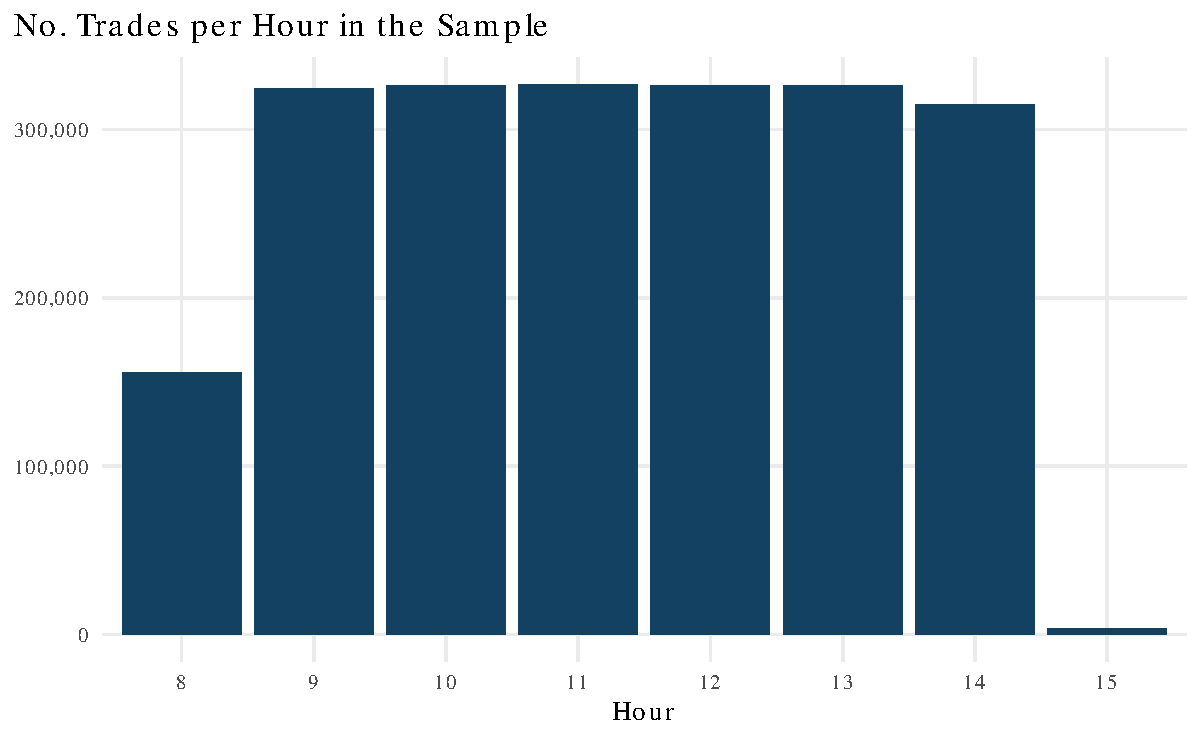
\includegraphics{01-Data-Prep-Elsevier_files/figure-latex/unnamed-chunk-27-1.pdf}

Most of the hours (9 - 14) have almost complete data. The hour number 8
has almost half the data points but that's natural since we only have
half an hour there. However, almost all of the log-returns for the
\texttt{15:00} mark seem to be missing. In normal business hours, we
have 6 hours and a half of market trading. If we have one-minute trades,
that means we should have \(6.5 * 60 + 1 = 391\) trades/day. The
\texttt{+1} in the equation comes from including the log-returns at
exactly \texttt{15:00} hours.

\begin{verbatim}
## [1] "2020-09-11 08:30:00 UTC" "2020-09-11 08:31:00 UTC"
## [3] "2020-09-11 08:32:00 UTC" "2020-09-11 08:33:00 UTC"
## [5] "2020-09-11 08:34:00 UTC" "2020-09-11 08:35:00 UTC"
\end{verbatim}

Therefore, we'll pad the time series with the mean log-return for each
half-hour.


\end{document}


